\documentclass{article}
\usepackage{fullpage}
\usepackage[utf8]{inputenc}
\usepackage{graphicx}
\usepackage[ngerman]{babel}
\usepackage{hyperref}
\usepackage{tabularx}
\usepackage{attachfile}
\usepackage{pdfpages}
\usepackage{siunitx}
\usepackage{caption} \captionsetup[table]{skip=10pt}
\usepackage[demo]{graphicx}
\usepackage{subfig}

\title{Ausarbeitung zu Schiefe Ebene (SEB)}
\author{Anfängerpraktikum Teil 1 \\Technische Universität München\\\\Leon Heiß, Paul Hildebrandt \\
Kurs 5, Gruppe 7, Team 19}
\date{21. Juni 2022}
\renewcommand*\contentsname{Inhaltsverzeichnis}

\renewcommand{\abstract}[1]{{ \noident {\bf\\Einleitung \\} #1 }}

\begin{document}

\maketitle

\large
\begin{center}
\textbf{Abstract}\\
\normalsize
\medskip
In diesem Versuch werden die Kräfte näher untersucht, die auf einen Körper wirken, der eine
schiefe Ebene hinuntergleitet. Dabei liegt der Fokus auf der Kräftezerlegung sowie der Bestimmung
des Haftreibungs- bzw. des Gleitriebungskoeffizienten.

\end{center}
\normalsize

\tableofcontents

\section{Grundlagen}
\subsection{Kräftezerlegung}

\begin{equation}
    F_{\bot} = F_g \cdot \cos(\alpha)
\end{equation}
\begin{equation}
    F_{\parallel} = F_g \cdot \sin(\alpha)
\end{equation}



\begin{figure}[hbt!]
\centering
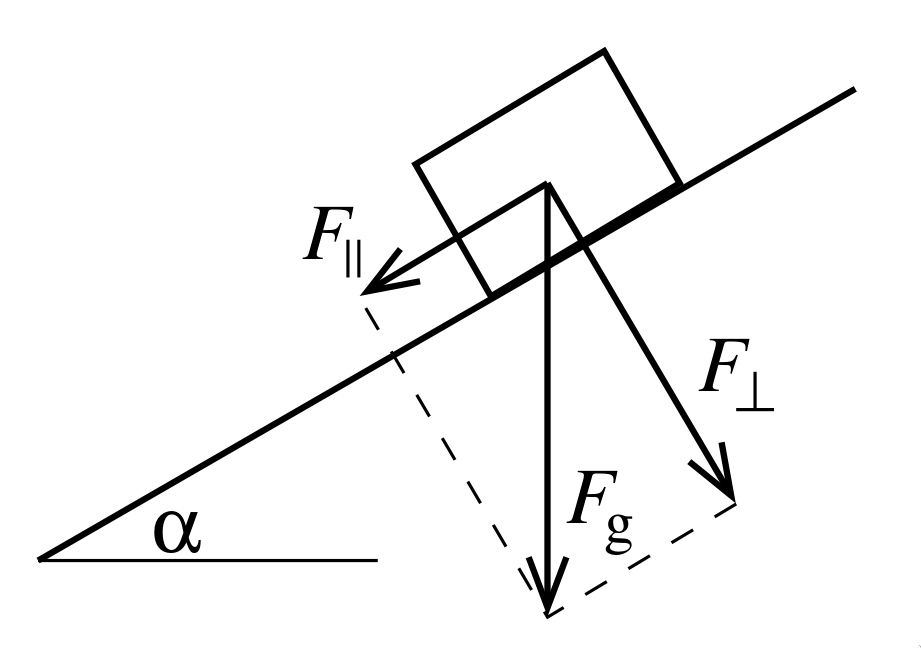
\includegraphics[width=200pt]{zerlegung.png}
\caption{Kräftezerlegung an der schiefen Ebene \cite{1}.}
\label{fig:length_eight_mouse}
\end{figure}

\subsection{Gleit- und Haftreibung}
\section{Überprüfen der Kräftezerlegung}
\subsection{Versuchsaufbau}
\begin{figure}
    \centering
    \subfloat[\centering Aufbau des Rutschers \cite{1}]{{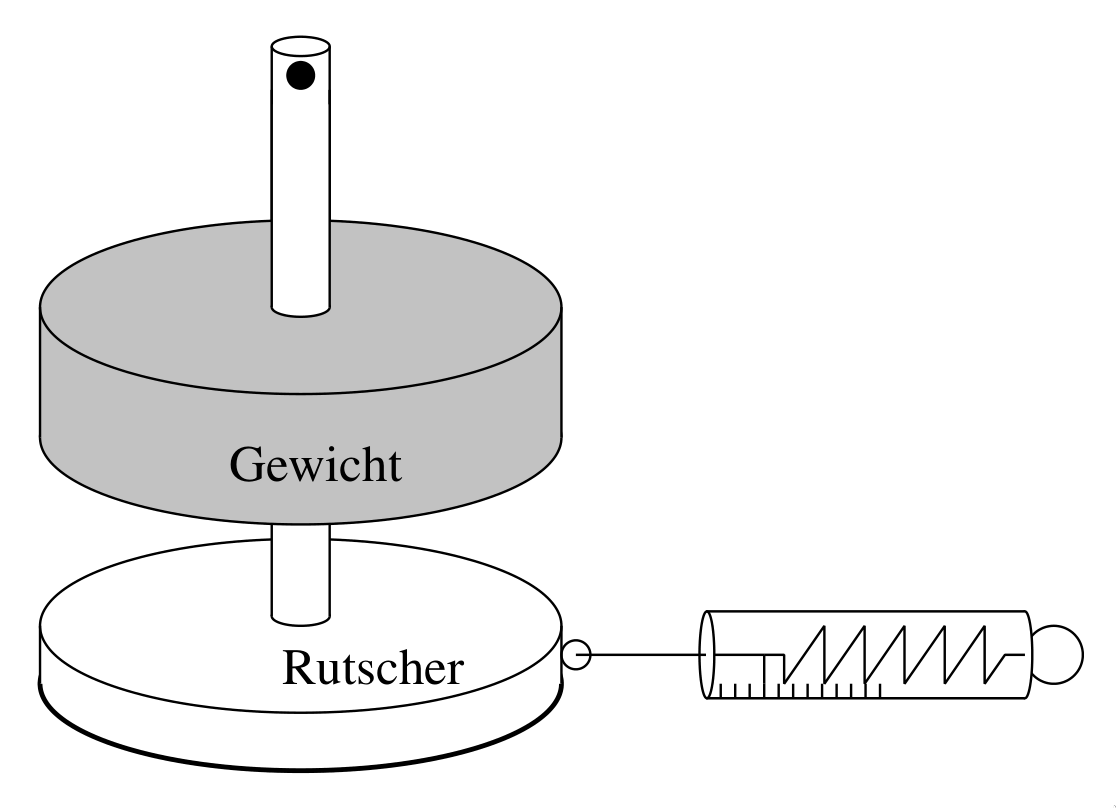
\includegraphics[width=5cm]{rutscher1.png} }}%
    \qquad
    \subfloat[\centering Versuchsaufbau zur Überprüfung der Kräftezerlegung \cite{1}]{{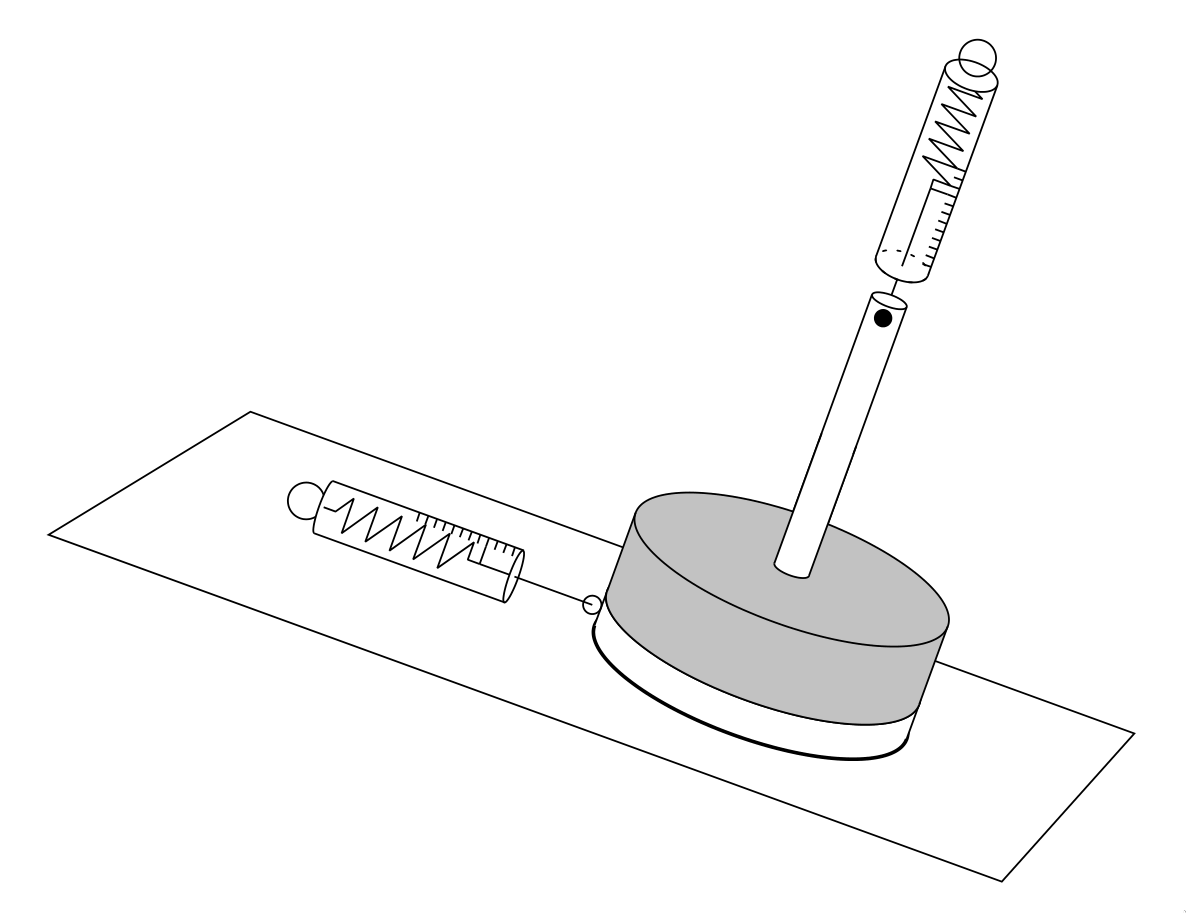
\includegraphics[width=5cm]{rutscher2.png} }}%
    \caption{}
    \label{fig:example}%
\end{figure}
\subsection{Auswertung}
\subsection{Fehlerrechnung}
\section{Bestimmung des Haftreibungskoeffizienten}
\subsection{Versuchsaufbau}
\subsection{Auswertung}
\section{Bestimmung des Gleitreibungskoeffizienten}
\subsection{Versuchaufbau}
\subsection{Auswertung}
\subsection{Fehlerrechnung}
\section{Literaturverzeichnis}
\begin{thebibliography}{9}
\bibitem{1}
Fakultät für Physik. \emph{Schiefe Ebene} (SEB. Technische Universität München. 24.06.2022.
\textbf{URL:} \url{https://www.ph.tum.de/academics/org/labs/ap/ap1/AKU.pdf}

\end{thebibliography}
\section{Anhang}
\subsection{Laborbuch}
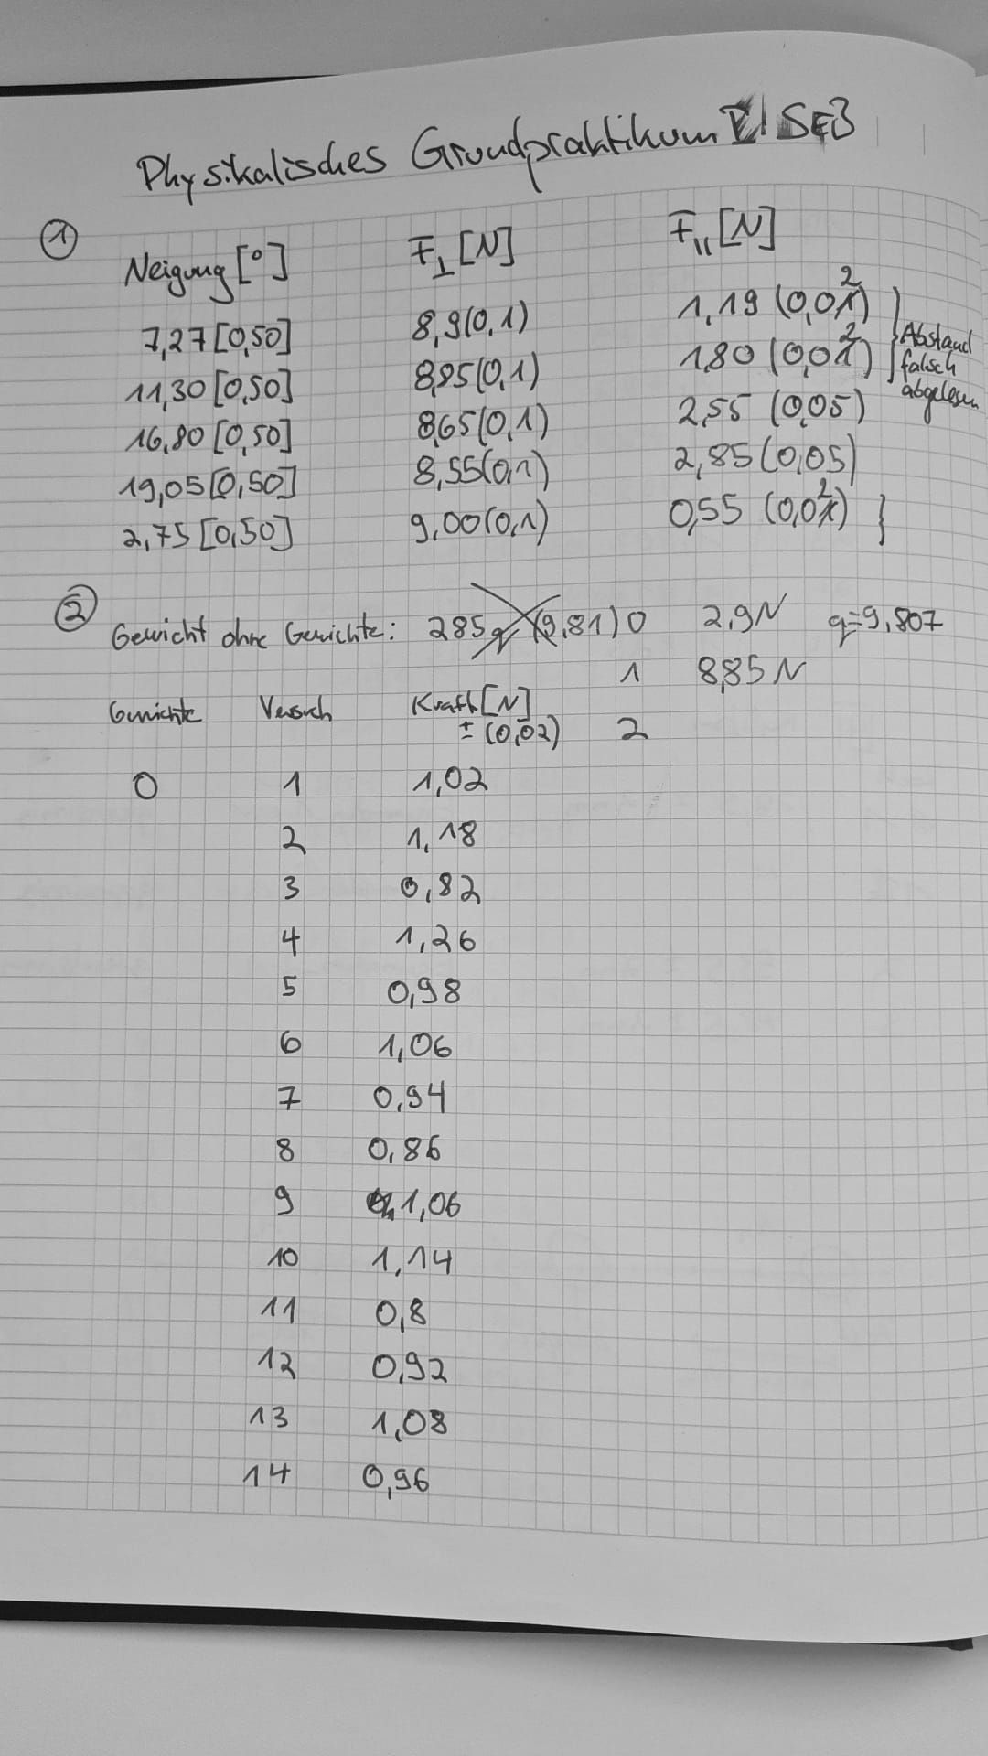
\includepdf[pages=-]{Protokoll.pdf}
\end{document}
